\documentclass[11pt]{article}
\usepackage{amsmath}
\usepackage{physics}
\usepackage{amssymb}
\usepackage{graphicx}
\usepackage{hyperref}
\usepackage{amsfonts}
\usepackage{cancel}
\usepackage{xcolor}
\hypersetup{
	colorlinks,
	linkcolor={black!50!black},
	citecolor={blue!50!black},
	urlcolor={blue!80!black}
}
\newcommand{\f}[2]{\frac{#1}{#2}}
\usepackage{newpxtext,newpxmath}
\usepackage[left=1.25in,right=1.25in,top=0.9in,bottom=0.9in]{geometry}
\usepackage{framed}
\usepackage{caption}
\usepackage{subcaption}





\begin{document}
\begin{center}
{\large \bf PH312: Physics of Fluids (Prof. McCoy) -- Reflection}\\
{ Huan Q. Bui}\\
Mar 17 2021
\end{center}

\begin{framed}
	\noindent Reflection on the readings:
	\begin{enumerate}
		\item Kundu \& Cohen 4.1 - 4.3; Tritton 5.4,
		\item Kundu \& Cohen 4.7
		\item  Kundu \& Cohen 4.10, 4.11; Tritton 5.6, 5.7
	\end{enumerate}
\end{framed}



I think we've finally gotten to the ``meat'' of fluid dynamics this week. Starting with conservation of mass, we then talked about conservation of momentum, and finally deriving the Navier-Stokes equation. \\

Even though I am familiar with a lot of these ideas (conservation laws, Newton's second law, and vector calculus), I find that putting them together to describe the same laws to describe fluid flow is actually very complicated and very subtle. One reason, I think, is that we have to work with fields in fluid dynamics (rather than point-particles), and so the calculus is much more involved. Another reason is interpreting the math. As we have seen, the calculus used to describe fluids is almost identical to that used in electromagnetism (things like conservation laws, Laplace/Poisson equations, stress tensor, etc. appear in both contexts), yet in fluid dynamics, we also talk about decomposing tensors into various parts responsible for different ``actions'' on our fluid element. Moreover, we have things like pressure, viscosity, and the Newtonian-ness of fluids, and so on. It's possible that (classical) electromagnetism is somewhat simpler than fluid dynamics because both electric and magnetic fields propagate at the speed of light, whereas the fluid flow speed can vary as a function of many factors. \\

I found this nice comparison between hydrodynamic and electromagnetic variables from \href{https://arxiv.org/ftp/arxiv/papers/1202/1202.4611.pdf}{arXiv:1202.4611}:

\begin{figure}[!htb]
	\centering
	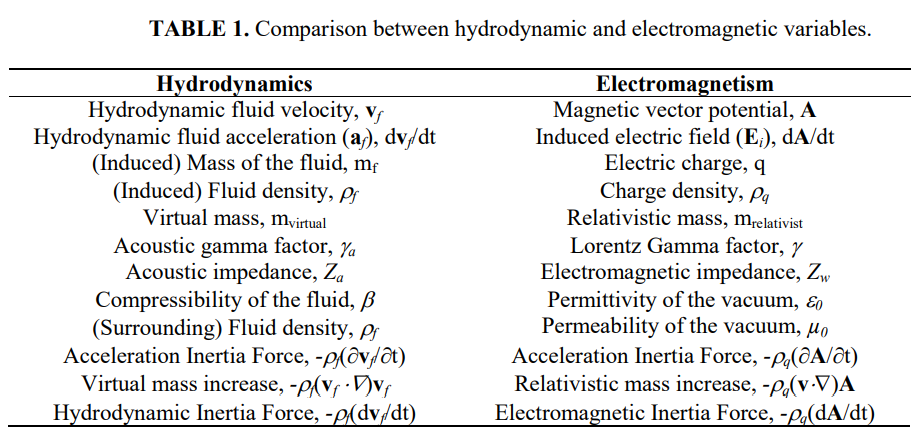
\includegraphics[scale=0.6]{compare}
\end{figure}




  
\end{document}




